%\documentclass[12pt, a3paper]{extarticle}
\documentclass[12pt, a4paper]{article}
\usepackage{graphicx, rotating, geometry}
\graphicspath{{./}}
\usepackage[utf8]{inputenc}
\usepackage{cite}
\usepackage{amsmath}
\usepackage{amsfonts}
\usepackage{mathtools}
\usepackage{hyperref}
\usepackage{listings}
\DeclarePairedDelimiter{\ceil}{\lceil}{\rceil}
\newcommand{\bo}{\textbf}
\newcommand{\ti}{\textit}
\newcommand{\ul}{\underline}

\lstdefinelanguage{solidity}{
  keywords={break, case, catch, continue, debugger, default, delete, do, else, finally, for, function, if, in, instanceof, new, return, switch, this, throw, try, typeof, var, void, while, with, contract, view, public, constructor, uint, pragma, const, module},
  morecomment=[l]{//},
  morecomment=[s]{/*}{*/},
  morestring=[b]',
  morestring=[b]",
  sensitive=true
}

\usepackage{color}

\definecolor{mygreen}{rgb}{0,0.6,0}
\definecolor{mygray}{rgb}{0.5,0.5,0.5}
\definecolor{mymauve}{rgb}{0.58,0,0.82}

\lstset{ 
  backgroundcolor=\color{white},   % choose the background color; you must add \usepackage{color} or \usepackage{xcolor}; should come as last argument
  basicstyle=\footnotesize,        % the size of the fonts that are used for the code
  breakatwhitespace=false,         % sets if automatic breaks should only happen at whitespace
  breaklines=true,                 % sets automatic line breaking
  captionpos=b,                    % sets the caption-position to bottom
  commentstyle=\color{mygreen},    % comment style
  deletekeywords={...},            % if you want to delete keywords from the given language
  escapeinside={\%*}{*)},          % if you want to add LaTeX within your code
  extendedchars=true,              % lets you use non-ASCII characters; for 8-bits encodings only, does not work with UTF-8
  firstnumber=1,                % start line enumeration with line 1000
  frame=single,	                   % adds a frame around the code
  keepspaces=true,                 % keeps spaces in text, useful for keeping indentation of code (possibly needs columns=flexible)
  keywordstyle=\color{blue},       % keyword style
  language=Octave,                 % the language of the code
  morekeywords={*,...},            % if you want to add more keywords to the set
  numbers=left,                    % where to put the line-numbers; possible values are (none, left, right)
  numbersep=5pt,                   % how far the line-numbers are from the code
  numberstyle=\tiny\color{mygray}, % the style that is used for the line-numbers
  rulecolor=\color{black},         % if not set, the frame-color may be changed on line-breaks within not-black text (e.g. comments (green here))
  showspaces=false,                % show spaces everywhere adding particular underscores; it overrides 'showstringspaces'
  showstringspaces=false,          % underline spaces within strings only
  showtabs=false,                  % show tabs within strings adding particular underscores
  stepnumber=1,                    % the step between two line-numbers. If it's 1, each line will be numbered
  stringstyle=\color{mymauve},     % string literal style
  tabsize=2,	                   % sets default tabsize to 2 spaces
  title=\lstname                   % show the filename of files included with \lstinputlisting; also try caption instead of title
}
\title{Blockchain Mid Term Solutions}
%\subtitle{Assignment 1}
\author{Mayank Sharma, 160392}
\date{February 14 2019}

\begin{document}
%\newcommand{\b}{\textbf}
\maketitle

\section{}
\begin{itemize}
		\item Increase the size of block: 
	\begin{itemize}
			\item Currently, the size of block is fixed, hence at max only a couple of thousand transactions can be included in a block. 
			\item Con: Larger blocks makes lesser number of miners/hashers to run as full nodes, hence causing the power to be centralized into some handful of pools. More data per block = more data to process for each node. This inevitably causes decentralization, and hence lowers the trust in bitcoin.
	\end{itemize}
		\item Decrease the difficulty to mine a block. 
	\begin{itemize}
			\item This causes more number of blocks to be mined per hour, and hence increases the number of transactions.
			\item Con: More number of forks may occur due to lower time to mine a block. It wastes hashing power and electricity too.
	\end{itemize}
\end{itemize}


\newpage
\section{}

\subsection{Output}
Below code is compiled using 
\begin{lstlisting}[language=bash]
g++ -Wall -L /usr/local/lib/  -o foobar foobar.cpp -lssl -lcrypto
\end{lstlisting}
\begin{lstlisting}
-----BEGIN PUBLIC KEY-----
MIIBIjANBgkqhkiG9w0BAQEFAAOCAQ8AMIIBCgKCAQEAvVDOs4Ewxh6273y4kjDk
ivURFbbK1iQEWeGsEQip4P40LS3SRulE//+CzV3Pr5ZlpqCl+9sEKW0S8hFdjiVF
NjpWImWYhLevIl4Ne0CV6uiSOGN5a45uTXzsgpElTZUxCMzT6wTtjKVxcRhplOSP
pToLG8I5iR0fIdLOGudoBZNRODItGotCoUG9bSqrJi10rTjrOowDIjJg4itsECbP
UkfoaGQZJjTi2s2/Jl2BILX3LESyT0jeSOptpKmYbl+KBIl/qXYQtzj2laBUkx+6
eVn3v0/xMfCk374rjrDkLs3wb1BGXiwmHirIYYo/NuQHZ/uqgYIrHGe/r9muCq98
sQIDAQAB
-----END PUBLIC KEY-----

SHA-256 Hashed and then Base58 Encoded Public Key = 
G78Kz4Ra5srKvNr1Fp1dqoEWuqnXaHGZabwKyxcyM2G1
\end{lstlisting}
\begin{lstlisting}[language=c++]{foobar.cpp}
#include <iostream>
#include <cstdio>
#include <cstring>
#include <string>
#include <vector>
#include <memory>
#include <assert.h>
#include <openssl/conf.h>
#include <openssl/evp.h>
#include <openssl/err.h>
#include <openssl/pem.h>
#include <openssl/crypto.h>
#include <openssl/sha.h>
typedef std::vector<uint8_t> uint8_vector_t;

// Reference : https://github.com/bitcoin/bitcoin/blob/master/src/base58.cpp
// This is take from original source code for bitcoin, it's just a helper function
static const char* pszBase58 = "123456789ABCDEFGHJKLMNPQRSTUVWXYZabcdefghijkmnopqrstuvwxyz";
std::string EncodeBase58(const unsigned char* pbegin, const unsigned char* pend)
{
	// Skip & count leading zeroes.
	int zeroes = 0;
	int length = 0;
	while (pbegin != pend && *pbegin == 0) {
		pbegin++;
		zeroes++;
	}
	// Allocate enough space in big-endian base58 representation.
	int size = (pend - pbegin) * 138 / 100 + 1; // log(256) / log(58), rounded up.
	std::vector<unsigned char> b58(size);
	// Process the bytes.
	while (pbegin != pend) {
		int carry = *pbegin;
		int i = 0;
		// Apply "b58 = b58 * 256 + ch".
		for (std::vector<unsigned char>::reverse_iterator it = b58.rbegin(); (carry != 0 || i < length) && (it != b58.rend()); it++, i++) {
			carry += 256 * (*it);
			*it = carry % 58;
			carry /= 58;
		}

		assert(carry == 0);
		length = i;
		pbegin++;
	}
	// Skip leading zeroes in base58 result.
	std::vector<unsigned char>::iterator it = b58.begin() + (size - length);
	while (it != b58.end() && *it == 0)
		it++;
	// Translate the result into a string.
	std::string str;
	str.reserve(zeroes + (b58.end() - it));
	str.assign(zeroes, '1');
	while (it != b58.end())
		str += pszBase58[*(it++)];
	return str;
}
std::string EncodeBase58(const std::vector<unsigned char>& vch)
{
	return EncodeBase58(vch.data(), vch.data() + vch.size());
}
void setup_context() {
	ERR_load_crypto_strings();
	OpenSSL_add_all_algorithms();
	OPENSSL_config(NULL);
	RSA_new();
}

void cleanup_context(){
	CONF_modules_free();
	CRYPTO_cleanup_all_ex_data();
	ERR_free_strings();
	EVP_cleanup();
}
int main() {
	// Setup the OpenSSL Context with various algorithms
	setup_context();
	int ret = 0;
	RSA *rsa = NULL;
	BIGNUM *bne = NULL;

	// set e
	bne = BN_new();
	ret = BN_set_word(bne, RSA_F4);
	assert(ret == 1);

	// generate key.
	rsa = RSA_new();
	ret = RSA_generate_key_ex(rsa, 2048 , bne , NULL);
	assert(ret == 1);
	// get rid of the bignum.
	BN_free(bne);

	// Declare a new Private Key and fill with random new value
	EVP_PKEY* privateKey = EVP_PKEY_new();
	assert (privateKey != NULL);
	// Use the declared rsa object to generate a private key
	EVP_PKEY_assign_RSA(privateKey, rsa);

	// dump public key in DER format
	uint8_t* derBuffer = NULL;
	auto derBufferLen = i2d_RSA_PUBKEY(rsa, &derBuffer);
	EVP_PKEY* publicKey = EVP_PKEY_new();
	assert (publicKey != NULL);
	// Use the rsa object to generate the corresponding public key for privateKey 
	EVP_PKEY_assign_RSA(publicKey, rsa);
	assert (derBufferLen > 0);

	// Write the un-encrypted (not password protected) private key to stdout
	PEM_write_PrivateKey(stdout, privateKey, NULL, NULL, 0, NULL, NULL);
	// Write the public key to stdout 
	PEM_write_PUBKEY(stdout, publicKey);
	unsigned char hash[SHA256_DIGEST_LENGTH];

	// Find the SHA256 Hash of the public key
	SHA256_CTX sha256;
	SHA256_Init(&sha256);
	SHA256_Update(&sha256, &derBuffer[0], derBufferLen);
	SHA256_Final(hash, &sha256);

	std::vector<unsigned char> temp;
	for(int i = 0; i < SHA256_DIGEST_LENGTH; i += 1)
		temp.push_back(hash[i]);
	std::cout << "SHA-256 Hashed and then Base58 Encoded Public Key = " << std::endl;
	// Base58 Encode the hash of public key 
	std::cout << EncodeBase58(temp) << std::endl;

	free(derBuffer);
	cleanup_context();
}
\end{lstlisting}


\newpage
\section{}
The statement \ti{ “In bitcoin blockchain, double-spend attack is never possible” } is false. Double-spending attacks however uncommon can be possible due to the following two reasons:

\begin{itemize}
	\item For the merchants accepting 0-confimation transactions, a double-spending is highly probable (called race attack). The person (say Alice) paying to the merchant for a service can send a valid transaction to merchant while also sending a conflicting transaction spending the coin to himself to the rest of network. \\ \\
		Then, any malicious node (which can be controlled by Alice) can cause the correct transaction to not be included in the new block, whereas a double-spending transaction will get processed and be included in the next block by such a node.
		\item \bo{51 \% attack: } A single large enough node which controls 51\% hash rate of the network can cause his own privately mined fork to grow to a large extent and then publishing his own mined blocks to the main chain.
			Moreover, since such an entity has large hashing power, he can mine blocks at a much faster rate thereby confirming the double-spending transactions faster than any heahtly node can. The moment of relief is that such an attack is highly improbable.  
\end{itemize}

\newpage
\section{Selfish Mining}

\subsection{}
A selfish miner doesn't gets benefitted directly by mining selfishly, Instead, what he relies upon is wasting the hash/compute power of other miners to effectively gain advantage over them. \\ \\
By broadcasting a block sometime later, he makes the other miners mine for the same block which has been found out by him. So, while he's trying to find a newer block, the others are just wasting their efforts on the previous block, thereby getting an unfair advantage over others.
\subsection{}
Firstly, a globally synchronizable time is not achievable. Secondly, The miner who is mining the block is the master of the block at that time, so he can decide to forge a fake time on the new block. This will further cause problems with the blockchain. 

\newpage
\section{}
\subsection{}
Probability to solve hash-puzzle  $ = p$ \\ 
Ways to choose $k$ miners out of $n$ = $ \binom{n}{k}$ \\
For k miners, prob. to solve hash-puzzle simultaneously 
\begin{align}
	=& \binom{n}{k} (p)^k (1-p)^{n-k}
\end{align}
\subsection{}
Consider the exponential distribution with Probability density function (pdf)
\begin{align}
	\text{pdf} =& \lambda \exp{-\lambda x} 
\end{align}


\newpage
\section{BoyCott possible?}

Bitcoin has no mechanism to penalize any malicious user, thereby a scheme wherein we BoyCott some node is not possible. Even if such a scheme were possible, the malicious person can simply create a new wallet address by generating a new public/private key pair and using that to mine blocks.
Blockchain also doesn't store any information related to the IP of miners hence an IP ban is out of the way too. Hence, boycotting any miner's chain can't prevent them from creating a new identity (priv/pub key pair) and start performing malicious behaviour again. \\ \\ 
Instead, what blockchain relies upon for promoting normal behaviour is the game-theoretic possibilities which a node can use to maximize his profits. Each node picks a strategy  to maximize its payoff by taking into account the other nodes' potential strategies. Every node is assumed to act according to its incentives, we can't split nodes into malicious or benign.


\newpage
\section{Mining Pools}
The designer can change the hash puzzle problem from "Find the nonce such that the Hash belongs to the target space " to the new hash puzzle "Find the nonce and such that the hash of the digital signature belongs to a certain target space".  \\  \\
This setting automatically highly discourages a minig pool setup because calculating the digital signature requires the knowledge of private key of pool manager to all the nodes participating in the pool. 
\\ \\
Any malicious person can steal the private key and use this to steal the money from the bitcoin wallet to which a block reward payment goes to on successful mining of a block. This way, a mining pool get split into a few trusted nodes only.


\newpage
\section{Solidity Program}
\begin{lstlisting}[language=solidity]{MyFirstContract.sol}
pragma solidity ^0.5.0;

// Create a new Contract
contract MyFirstContract {
	// Declare balance as a uint (256 bit unsigned int) 
	uint balance;

	// View function getBalance - View functions promise to not make any changes to state of contract 
	// Return Value Type (uint) 
	function getBalance() public view returns (uint) {
		return balance;
	}

	// constructor sets balance 
	constructor() public {
		balance = 100;
	}
}
\end{lstlisting}

\begin{lstlisting}[language=solidity]{3\_deploy\_contracts.js}
const MyFirstContract = artifacts.require("./MyFirstContract.sol");

// Export the deployer of  MyFirstContract 
module.exports = function(deployer) {
	// Deploy the MyFirstContract on Network
	deployer.deploy(MyFirstContract);
}
\end{lstlisting}

\begin{lstlisting}[language=solidity]{MyFirstContractTest.js}
const MyFirstContract = artifacts.require("MyFirstContract") 

contract('MyFirstContract', () => {
	it("Should always return 100 when getBalance() is called.", async () => {
		const firstContractInstance = await MyFirstContract.deployed()
		const balance = await firstContractInstance.getBalance()
		assert.equal(balance, 100,
			"Oops! Default balance wasn't 100");
		
	})
})
\end{lstlisting}
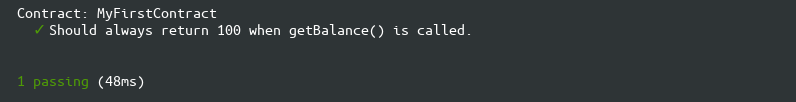
\includegraphics[scale=0.5]{test.png}
\begin{lstlisting}[language=solidity]{truffle-config.js}
module.exports = {
  networks: {
    // Useful for testing. The `development` name is special - truffle uses it by default
    // if it's defined here and no other network is specified at the command line.
    // You should run a client (like ganache-cli, geth or parity) in a separate terminal
    // tab if you use this network and you must also set the `host`, `port` and `network_id`
    // options below to some value.
    //
		 development: {
			host: "127.0.0.1",     // Localhost (default: none)
			port: 8545,            // Standard Ethereum port (default: none)
			network_id: "*",       // Any network (default: none)
		 },

  },

  // Set default mocha options here, use special reporters etc.
  mocha: {
  },

  // Configure your compilers
  compilers: {
    solc: {
    }
  }
}
\end{lstlisting}

\newpage
\section{Pros and Cons}
\subsection{Advantages of Bitcoin over Ethereum}\\
\begin{itemize}
	\item Ethereum doesn't have a cap on number of coins, which means it has high inflation.
	\item Bitcoin uses UTXO model which has more scalability since transactions can be processed in parallel since they all refer to independent inputs.
	\item Bitcoin is much more widely accepted as compared to Ethereum. Many online wallets and merchants only allow payments via BTC, and not ether.
	\item Bitcoin is digital currency and has more market value than Ethereum.
	\item Ethereum's blockchain takes up A LOT of space. Over 1GB is added every month.
\end{itemize}
\subsection{Advantages of Ethereum over Bitcoin}\\
\begin{itemize}
	\item Much faster transactions and their processing (12 seconds compared to 10 minutes for 1 block).
	\item Ethereum has a built in Virtual Machine and Ethereum is Turing Complete.
	\item Ethereum uses Account Based Model which provides advantages like larger space saving, simplicity and familiarity.
	\item Ethereum allows the use of smart contracts which has multiple advantages
	\item Ethereum is an open-ended decentralized platform which enables the creation of Distributed Applications over it's network.

\end{itemize}

\end{document}









